\begin{figure*}[t]
  \centering
  \begin{subfigure}{0pt}\phantomsubcaption\label{fig:synth-f1}\end{subfigure}%
  \begin{subfigure}{0pt}\phantomsubcaption\label{fig:synth-f2}\end{subfigure}%
  \begin{subfigure}{0pt}\phantomsubcaption\label{fig:synth-f3}\end{subfigure}%
  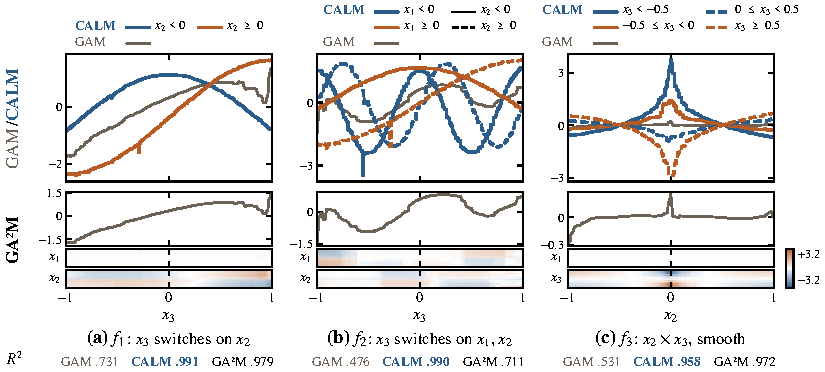
\includegraphics[width=\linewidth]{images/custom-visuals/synthetic}
  \caption{
    Cases~1 to 3 (one column each) of Section~\ref{sec:explanatory_example}.
    Top: \method{}'s curves, one per region, over the GAM's single curve (gray).
    Bottom: the \gamm{}'s main curve alongside its two heatmaps.
    Under each column: the mean $R^2$ over 5 folds (Table~\ref{tab:explanatory-example-r2}), with \method{} at depth~2; $f_1$'s panel is drawn at depth~1.
    }
  \label{fig:shape_functions}
\end{figure*}

We evaluate \method{} on three synthetic regression datasets and 24 public real-world tabular datasets, 10 for classification and 14 for regression.
Every experiment runs \method{} with its default configuration: XGBoost as the reference model in Step 1(a), PDP-based heterogeneity to propose the trees in Step~1(b),  EBM to fit the curves in Step~2, and the default hyperparameters of Section~\ref{subsec:model-overview} for Steps~1(b)--(c).
No hyperparameter is tuned per dataset, for both \method{} and the baselines.
Appendix~\ref{app:detailed-experiments} provides full implementation details.
Results are reported as the mean $\pm$ standard deviation over 5-fold cross-validation.

\subsection{Synthetic example}\label{sec:explanatory_example}

On three synthetic regression datasets, we compare \method{} against EBM, as the GAM, and EB$^2$M, as the \gamm{}.
In all three, the dataset consists of 1{,}000 draws of three independent features $x_i \sim \mathcal{U}(-1, 1)$; only the target $y=f_k(\xb)$ varies and each $f_k$ contains a different interaction structure:
in Case~1, a conditional interaction of two features (one curve of $x_3$ per sign of $x_2$), which both \method{} and a \gamm{} can express;
in Case~2, a conditional interaction of three features (one curve of $x_3$ per signs of $x_1$ and $x_2$), which only \method{} can express;
in Case~3, a general interaction of two features (a full $x_2$–$x_3$ term), which a \gamm{} can express and \method{} can only approximate by regions.
The targets are
\begin{align*}
f_1(\xb) &= x_1^2 + \log|x_2| + 2\sin(\tfrac{\pi}{2} x_3)\,\mathbf{1}_{x_2 \geq 0} + 2\cos(\tfrac{\pi}{2} x_3)\,\mathbf{1}_{x_2 < 0}, \\
f_2(\xb) &= x_1^2 + \log|x_2| + 2\sin(\omega x_3)\,\mathbf{1}_{x_2 \geq 0} + 2\cos(\omega x_3)\,\mathbf{1}_{x_2 < 0}, \quad \omega = \tfrac{\pi}{2}\,\mathbf{1}_{x_1 \geq 0} + 2\pi\,\mathbf{1}_{x_1 < 0}, \\
f_3(\xb) &= x_1^2 + \log|x_2| \sin(\tfrac{\pi}{2} x_3).
\end{align*}
Figure~\ref{fig:shape_functions} gives the $R^2$ of each model and Table~\ref{tab:explanatory-example-r2} (Appendix~\ref{app:synthetic}) its spread over the folds.

\textbf{Case 1.}
The GAM averages the sine and cosine modes of $x_3$ into one curve (Fig.~\ref{fig:synth-f1}, gray) and reaches $R^2 = 0.731$.
Both the \gamm{} and \method{} capture the switch on the sign of $x_2$, with near-perfect accuracy ($0.979$ and $0.991$).

\textbf{Case 2.}
The GAM merges the four modes of $x_3$ into one curve, limiting its accuracy to $R^2 = 0.476$.
The \gamm{} can only approximate the three-feature switch with its $x_1$–$x_3$ and $x_2$–$x_3$ surfaces and reaches $0.711$, while \method{} conditions $x_3$ on both signs and reaches $0.990$.

\textbf{Case 3.}
Averaged over $x_3$, the effect of $x_2$ cancels, so the GAM's curve of $x_2$ is nearly flat and its accuracy low ($R^2 = 0.531$).
The \gamm{} captures the product in its $x_2$–$x_3$ surface ($0.972$).
\method{} approximates it by splitting $x_3$ into four ranges, each with its own curve of $x_2$, and still reaches $0.958$, slightly below the \gamm{}.

\textbf{Interpretability.}
In every case, the \gamm{} spreads the effect of one feature over three views, its main curve and two heatmaps, which the reader must combine to draw conclusions (Fig.~\ref{fig:shape_functions}, bottom).
\method{} shows the same effect as a few 1D curves, each labelled by the condition that selects it (Fig.~\ref{fig:shape_functions}, top), so the questions P1--P3 of Section~\ref{subsec:interpretability-properties} are answered at a glance.
